\documentclass[norsk,a4paper,12pt]{article} 
\usepackage[norsk]{babel} 
\usepackage[T1]{fontenc} %for å bruke æøå 
\usepackage[utf8x]{inputenc} 
\usepackage{graphicx} %for å inkludere grafikk 
\usepackage{verbatim} %for å inkludere filer med tegn LaTeX ikke liker 
\usepackage{amsfonts} 
\usepackage{amsmath} 
\usepackage{amssymb} 
%\usepackage{savesym} 
%\savesymbol{square} 
\bibliographystyle{plain} 
\usepackage{float} 
%\usepackage{SIunits} 
\usepackage{textcomp} 
\usepackage{parskip} 
\usepackage{array} 
%\usepackage[framed]{mcode} 
\usepackage[margin=2.3cm]{caption}
\usepackage{listings}

\begin{document}

\title{AST5220 Cosmology II: Milestone 3}
\author{Peder Forfang}
\maketitle


\section{The evolution of structures in the universe}

The Cosmic Microwave Background (CMB) anisotropies is an important source of information on the history of the Universe and since first discovered has been a large research field in cosmology. This report is the 3rd part of a project concerning calculation of the CMB spectrum. To get the full picture, the other parts of the project should be taken into account. Here we will look at how small fluctuations in the baryon-photon-dark-matter fluid grow from shortly after inflation until today. We will take into account  photons, baryons and dark matter, and only temperature fluctuations. Thus neglecting neutrinos and polarization. To study these fluctuations we will construct a two-dimensional grid in time and Fourierscale, x and k, for each of the main physical quantities of interest; the gravitational potentials $\phi(x,k)$ and $\psi(x,k)$, density perturbations $\delta(x,k)$ and $\delta_b(x,k)$, velocities $v(x,k)$ and $v_b(x,k)$, and photon perturbation $\Theta_l(x,k)$ and their derivatives. The report contains one plot of each of the physical quantities as function of x for six different k's, chosen such that each of the main regimes are shown; large scales, intermediate scales and small scales.

Full equation set: 

\begin{equation}
 \Theta_0' = -\frac{ck}{H_p}\Theta_1 - \phi'
\end{equation}


\begin{equation}
 \Theta_1' = \frac{ck}{3H_p}\Theta_0 - \frac{2ck}{3H_p}\Theta_2 + \frac{ck}{3H_p}\psi + \tau'[\Theta_1 + \frac{1}{3}v_b]
\end{equation}

\begin{equation}
 \Theta_l' = \frac{lck}{(2l +1)H_p}\Theta_{l-1} - \frac{(l+1)ck}{(2l +1)H_p}\Theta_{l+1} + \tau'[\Theta_l + \frac{1}{10}\Theta_l \delta_{l,2}]
\end{equation}

where $ 2 \leq l < l_{max} $ in $ \delta_{l,2} $.

\begin{equation}
 \Theta_l' = \frac{ck}{H_p}\Theta_{l-1} - c\frac{l+1}{H_p\eta(X)}\Theta_l + \tau'\Theta_l
\end{equation}

where $l = l_{max}$.

\begin{equation}
 \delta' = \frac{ck}{H_p}v - 3\phi'
\end{equation}

\begin{equation}
 v' = -v-\frac{ck}{H_p}\psi
\end{equation}

\begin{equation}
 \delta_b = \frac{ck}{H_p}v_b - 3\psi'
\end{equation}

\begin{equation}
 v_b' = -v_b - \frac{ck}{H_p}\psi + \tau'R(3\Theta_1 + v_b)
\end{equation}

\begin{equation}
 \phi' = \psi - \frac{c^2k^2}{3H_p^2}\phi + \frac{H_0^2}{2H_p^2}[\Omega_m a^{-1}\delta + \Omega_b a^{-1}\delta_b + 4\Omega_ra^{-2}\Theta_0]
\end{equation}

\begin{equation}
 \psi = -\phi - \frac{12H_0^2}{c^2k^2a^2}\Omega_r\Theta_2
\end{equation}

\begin{equation}
 R = \frac{4\Omega_r}{3\Omega_b a}
\end{equation}


The equations for the physical quantities and their respective initial conditions are obtained by deriving the linearized Einstein and Boltzmann equations for photons, baryons and dark matter. In this report however, we will concern ourselves only with solving these equations numerically. The choice of initial conditions are decided through our definition of the gravitational potential $\phi$. Since our equations are linear however, we simply set $\phi(k,0)=1$, and in the end multiply the solution with the power spectrum we want. 

Initial conditions:

\begin{equation}
 \phi = 1
\end{equation}

\begin{equation}
 \delta = \delta_b = \frac{3}{2}\phi
\end{equation}

\begin{equation}
 v = v_b = \frac{ck}{2H_p}\phi
\end{equation}

\begin{equation}
 \Theta_0 = \frac{1}{2}\phi
\end{equation}

\begin{equation}
 \Theta_1 = \frac{ck}{6H_p}\phi
\end{equation}

\begin{equation}
 \Theta_2 = -\frac{20ck}{45H_p\tau'}\Theta_1
\end{equation}

\begin{equation}
 \Theta_l = -\frac{l}{2l + 1}\frac{ck}{H_p\tau'}\Theta_{l-1}
\end{equation}

In the beginning the optical depth $\tau$ is very large and $ck/H_p\tau'$ is small. It makes some of our system of equations numerically unstable and quite unpleasant to work with. We call this epoch the tight coupling regime. By tweeking a couple of our equations we can avoid any problems.

Tight coupling equations:

\begin{equation}
 q = \frac{-[(1-2R)\tau' + (1+R)\tau''](3\Theta_1 + v_b) - \frac{ck}{H_p}\psi + (1-\frac{H_p'}{H_p})\frac{ck}{H_p}(-\Theta_0 + 2\Theta_2) - \frac{ck}{H_p}\Theta_0'}{(1+R)\tau' + \frac{H_p'}{H_p}-1}
\end{equation}

\begin{equation}
 v_b' = \frac{1}{1 + R}[-v_b-\frac{ck}{H_p}\psi + R(q + \frac{ck}{H_p}(-\Theta_0 + 2\Theta_2) -\frac{ck}{H_p}\psi]
\end{equation}

\begin{equation}
 \Theta_1' = \frac{1}{3}(q-v_b')
\end{equation}

The expressions for the higher ordered photon moments during tight coupling are simply the same as the initial conditions,

\begin{equation}
 \Theta_2 = -\frac{20ck}{45H_p}\Theta_1
\end{equation}

\begin{equation}
 \Theta_l = -\frac{l}{2l + 1}\frac{ck}{H_p\tau'}\Theta_{l-1}
\end{equation}

The other quantities can be integrated as usual. The tight coupling regime lasts until certain conditions are met, namely $\tau' < 10$, $ck/H_p\tau'$ or x > x(start of recombination). When this condition is met we proceed to integrate the original equations. The results are shown in the figures below. Results from six different k values are shown in each plot, representing different scales. 

\begin{figure}[H] 
\begin{center} 
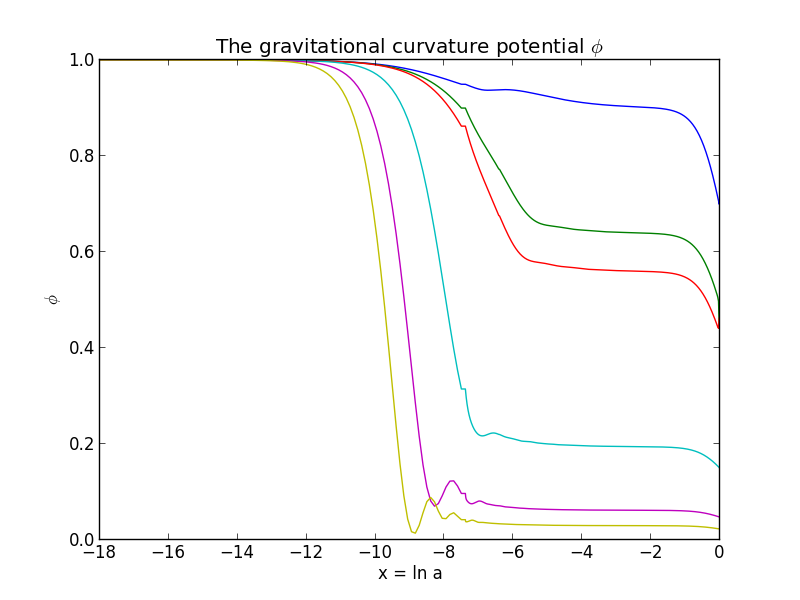
\includegraphics[scale=0.5]{phi.png} 
 

\caption{As mentioned earlier the initial condition of gravitational potential is chosen to be 1. At this time matter and radiation is gathered tightly. As the universe expands matter lumps together and the gravity gets more concentrated at small scales (yellow line). Gravity pulls and radiation push matter which is shown by the small oscillations at the bottom of the lines. As we reach matterdomination the potential is balanced by expansion. At the end the expansion dominates and the gravitational potential decrease again. The blue line represents the largest scales down to the smallest scale (yellow line). } 
\end{center} 
\end{figure}

\begin{figure}[H] 
\begin{center} 
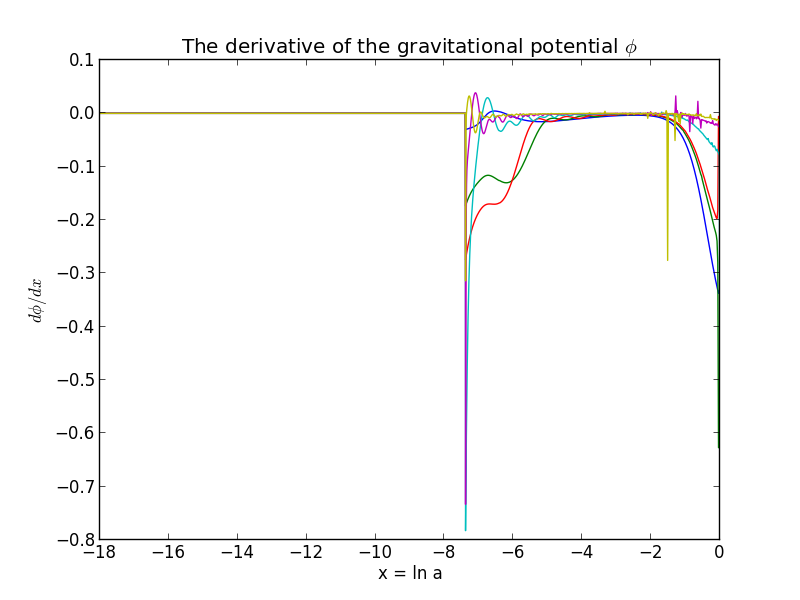
\includegraphics[scale=0.5]{dphi.png} 
 

 
\caption{} 
\end{center} 
\end{figure}

\begin{figure}[H] 
\begin{center} 
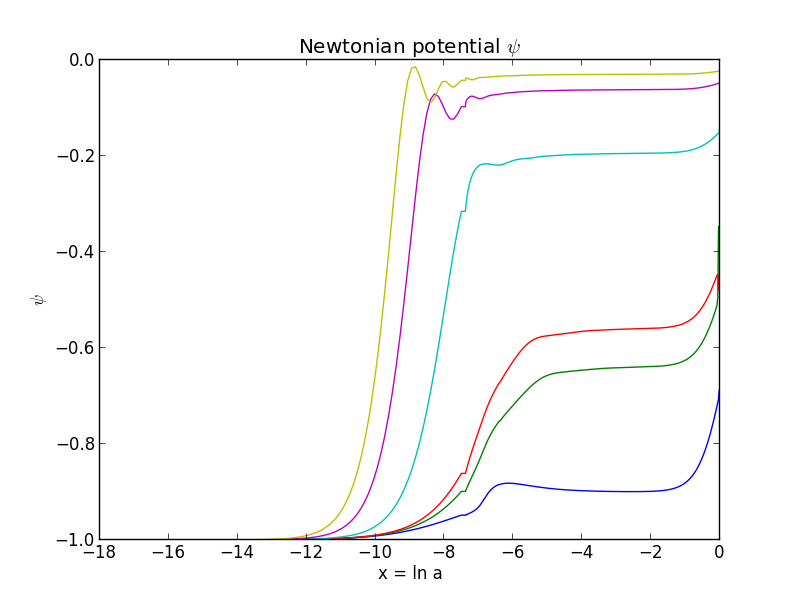
\includegraphics[scale=0.5]{psi.png} 
 

\caption{Exactly the opposite of the spacial curvature potential $\phi$, $\psi$ can be thought of as the curvature of time.} 
\end{center} 
\end{figure}

\begin{figure}[H] 
\begin{center} 
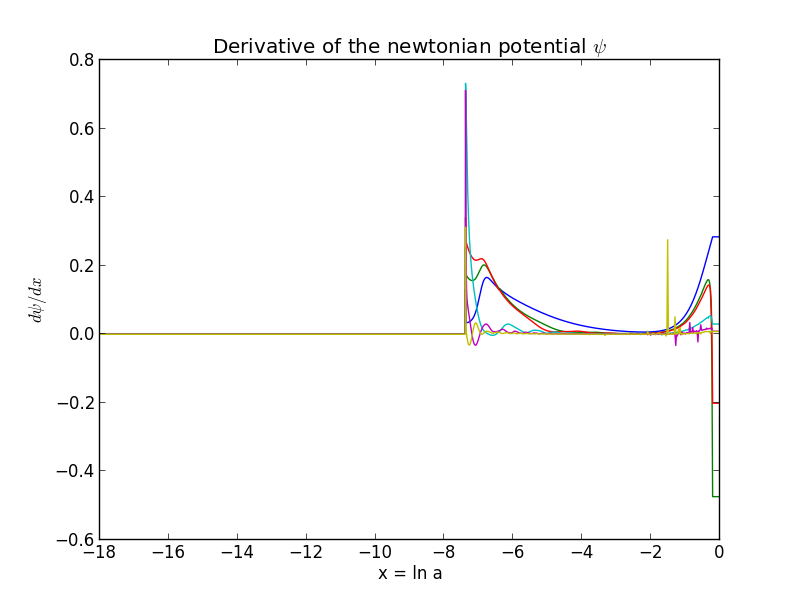
\includegraphics[scale=0.5]{dpsi.png} 
  
\caption{} 
\end{center} 
\end{figure}

The figures for the gravitational potentials $\phi$ and $\psi$ looks to be fine, but the derivatives reveal some slight weird behavior. This is caused by some numerical issues which could not be quite figured out and influenced some of the quantities below in a bad way.

\begin{figure}[H] 
\begin{center} 
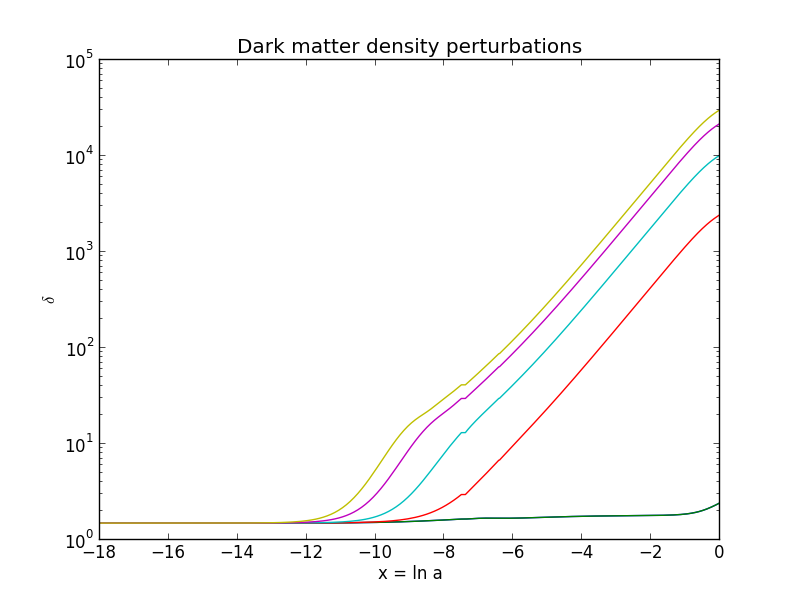
\includegraphics[scale=0.5]{delta.png} 
 

\caption{The dark matter perturbations are not affected photon pressure, but by the smaller amount of baryonic matter, thus it grows steadily.} 
\end{center} 
\end{figure}

\begin{figure}[H] 
\begin{center} 
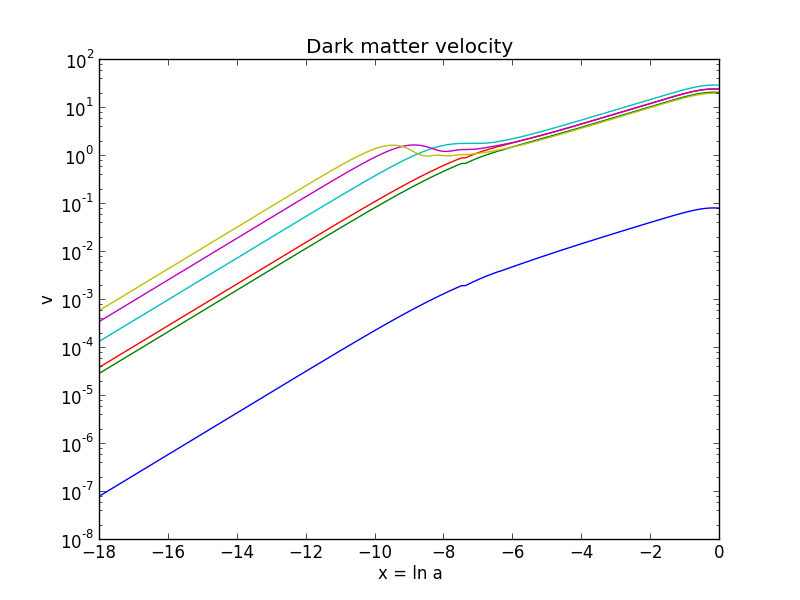
\includegraphics[scale=0.5]{v_log.png} 
 

\caption{The velocity of dark matter perturbations. As seen in the figure they are slightly affected by the oscillating barionic matter shown below.} 
\end{center} 
\end{figure}




\begin{figure}[H] 
\begin{center} 
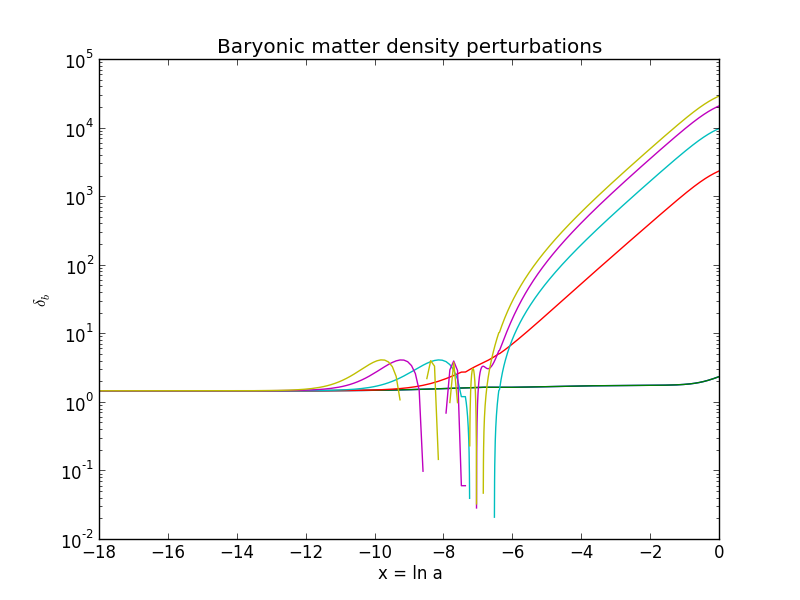
\includegraphics[scale=0.5]{delta_b.png} 
 

\caption{While dark matter does not feel radiation pressure, baryonic matter certainly do. Around matter-radiation equality and recombination these perturbations oscilliate with gravity and radiation pressure as a battery.} 
\end{center} 
\end{figure}

\begin{figure}[H] 
\begin{center} 
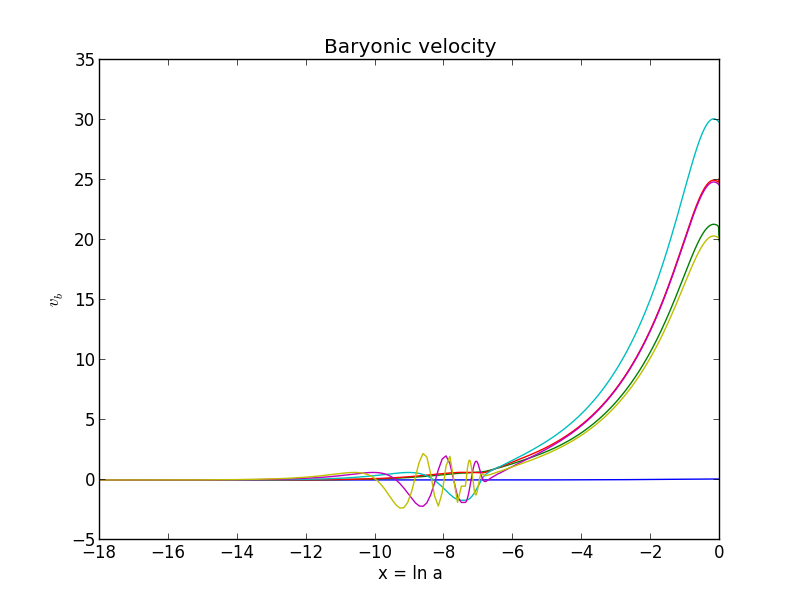
\includegraphics[scale=0.5]{v_b.png} 
 

\caption{The velocity of barionic perturbations. This velocity is relative to the expansion rate. Thus when the expansion is increasing the velocity will slow down.} 
\end{center} 
\end{figure}

\begin{figure}[H] 
\begin{center} 
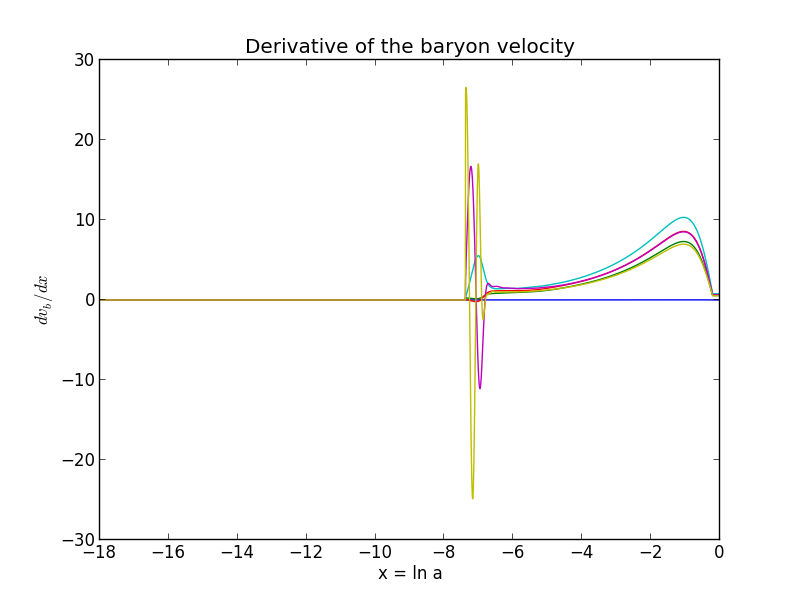
\includegraphics[scale=0.5]{dv_b.png} 
 

\caption{} 
\end{center} 
\end{figure}

\begin{figure}[H] 
\begin{center} 
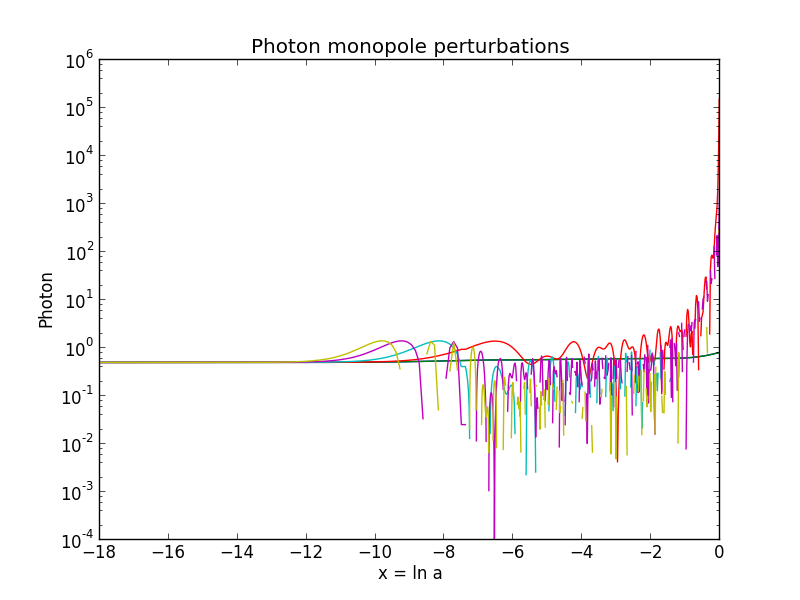
\includegraphics[scale=0.5]{photon.png} 
 

\caption{Normally the monopole of the photon perturbations can be interpreted as the average temperature of the CMB photons. Some numerical issues made a mess of it, sadly. } 
\end{center} 
\end{figure}

\begin{figure}[H] 
\begin{center} 
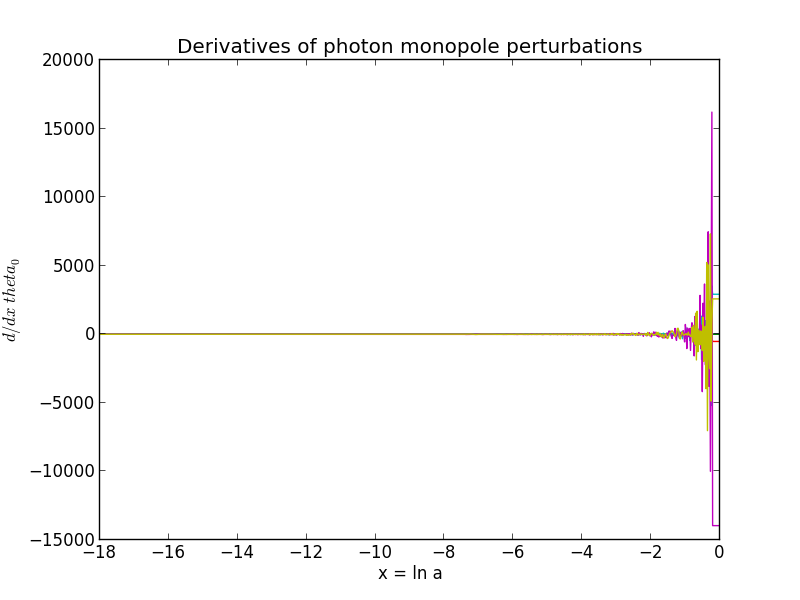
\includegraphics[scale=0.5]{dphoton.png} 
 

\caption{.} 
\end{center} 
\end{figure}


\end{document}